%% Numbers    checked
%% Spelling   checked
%% Acronyms   checked

\chapter{The Standard Model}
\label{chap:I-1-standard-model}

  The standard model provides a classification and description of the subatomic particles that compose our universe and their interactions. It describes both the particles of matter called fermions, which are subdivided among quarks and leptons, and the force carriers named bosons. Figure \ref{fig:I-1-sm-particles} illustrates the particle content of the standard model and the ways they are classified among types and generations. Quarks and leptons, and their antiparticles antiquarks and antileptons, are further divided into three generations with identical properties but increasing mass, from which the first constitutes the everyday matter while the two others, unstable, quickly decay towards lower generations. The interaction of fermions with each other is carried out through the exchange of bosons. Gluons are the carriers of the strong force and interact solely with themselves and quarks as described by quantum chromodynamics (QCD). The photon, responsible for electromagnetism couples to all charged particles while the $ W^\pm $ and $ Z $ bosons couple to all particles except gluons as described by the electroweak theory (EWK). Finally, the Higgs boson as previously stated is the manifestation of the Higgs mechanism at the origin of mass. \\

	\begin{figure}[h!]
		\centering
		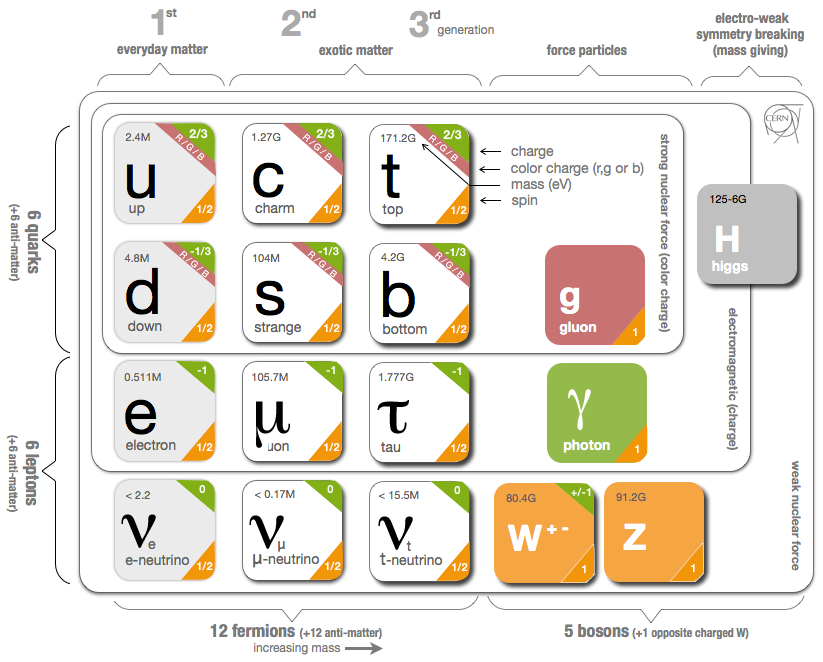
\includegraphics[width=\textwidth]{img/I-1-standard-model/sm-particles.png}
		\caption{Overview of the elementary particles as described by the standard model. Everyday matter is composed of the first generation of quarks and leptons to which two heavier generations are added. Gauge bosons or force particles are the carriers of the interactions between other particles. The Higgs boson is the manifestation of the mechanism that gives mass to particles [CERN].}
		\label{fig:I-1-sm-particles}
	\end{figure}

  Besides classifying particles, the standard model also provides a strong mathematical model built on top of quantum field theory and gauge invariance that yields an accurate representation of the fundamental processes of the universe. The gauge group of the theory is $ SU(3)_C \otimes SU(2)_L \otimes U(1)_Y $, where $ SU(3)_C $ and $ SU(2)_L \otimes U(1)_Y $ are respectively the symmetry groups of the QCD and EWK sectors. In this paradigm, quarks and leptons are represented as fermionic fields within the Lagrangian of the model while bosons arise from the invariance of the Lagrangian under local gauge transformations. \\

  \section{Gauge Invariance and Gauge Bosons}

    In the standard model, bosons are mathematical and physical objects that arise from the requirement of gauge invariance of the Lagrangian. This constraint translates the fact that the physics of the system does not change under an arbitrary phase change of the coordinate system. A local transformation of a fermionic field $ \psi $ under a gauge group $ G $  can be written as
    \begin{equation}
      \psi \rightarrow \psi' = \exp\left(- \frac{i}{2} g \alpha^k(x) T^k \right) \psi ,
    \end{equation}
    where $ g $ is the gauge coupling constant, $ \alpha^k(x) $ are the local rotation parameters, and $ T^k $ are the generators of the representation of $ G $. To preserve the invariance of the Lagrangian of a free massless field $ \psi $,
    \begin{equation}
      \mathcal{L} = i \bar{\psi} \gamma^\mu \partial_\mu \psi ,
    \end{equation}
    the partial derivate $ \partial_\mu $ must be rewritten as a covariant derivate to absorb the change in coordinates
    \begin{equation}
      D_\mu = \partial_\mu - \frac{i g}{2} W^k_\mu T^k ,
    \end{equation}
    where $ W^k_\mu $ are the emerging gauge fields associated to $ G $. The gauge invariant Lagrangian thus becomes
    \begin{equation}
      \mathcal{L} = i \bar{\psi} \gamma^\mu D_\mu \psi - \frac{1}{4} W^i_{\mu \nu} W^{i \mu \nu} ,
    \end{equation}
    where $ W^i_{\mu \nu} $ are the field strength tensors of the $ W^i_\mu $ gauge fields given by
    \begin{equation}
      W^i_{\mu \nu} = \partial_\mu W^i_\nu - \partial_\nu W^i_\mu - g \epsilon^{ijk} W^j_\nu W^k_\mu ,
    \end{equation}
    with $ \epsilon^{ijk} $ the totally antisymmetric tensor. From the necessity of the invariance of the theory under local transformations, a new massless gauge boson is associated to each generator of the adjoint representation of the symmetry group $ G $. Moreover, interaction terms between the fermionic field $ \psi $ and the gauge fields $ W^i_\mu $ as well as self-interacting gauge field terms have emerged. These are represented in Figure \ref{fig:I-1-diagram} which provides a schematic view of the processes at play using Feynman diagrams.

    \begin{figure}[h!]
      \centering
      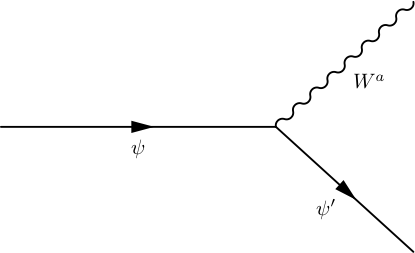
\includegraphics[width=0.49\textwidth]{img/I-1-standard-model/diagram-fermion-boson.png}
      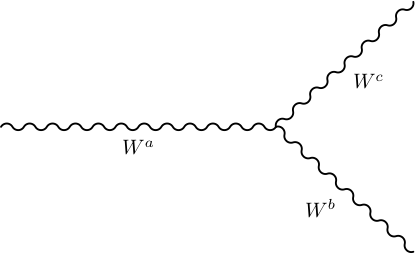
\includegraphics[width=0.49\textwidth]{img/I-1-standard-model/diagram-boson-boson.png}
      \caption{Feynman diagrams representing the interaction terms of the Lagrangian. Left: interaction between a fermion and a boson. Right: self-interaction of gauge bosons.}
      \label{fig:I-1-diagram}
    \end{figure}

  \section{Electroweak Theory}

    The gauge group of the EWK sector of the standard model is $ SU(2)_L \otimes U(1)_Y $ for which a transformation of a fermionic field $ \psi $ can be written as
    \begin{equation}
      \psi \rightarrow \psi' = \exp\left(- \frac{i}{2} g_W \Lambda^k(x) T^k \right) \exp\left(- \frac{i}{2} g_W' \alpha(x) Y \right) \psi ,
    \end{equation}
    where $ g_W $, $ \Lambda^k(x) $, and $ T^k $ are respectively the gauge coupling, local rotation parameters, and representation of the $ SU(2)_L $ weak isospin algebra and $ g_W' $, $ \alpha(x) $, and $ Y $ are their $ U(1)_Y $ hypercharge algebra counterparts. The corresponding covariant derivate is
    \begin{equation}
      D_\mu = \partial_\mu - \frac{i g_W}{2} W^k_\mu T^k - \frac{i g_W'}{2} B_\mu Y ,
    \end{equation}
    where $ W^k_\mu $ and $ B_\mu$ are the emerging gauge fields associated to $ SU(2)_L $ and $ U(1)_Y $. \\

    Each fermion can couple differently to the gauge fields according to the representation of the $ SU(2)_L $ group they are part of. To determine the coupling constants it is important to separate each fermionic field into its left-handed and right-handed components such that
    \begin{equation}
      \psi = \psi_L + \psi_R \equiv \gamma^L \psi + \gamma^R \psi ,
    \end{equation}
    with
    \begin{align}
      \gamma^{L/R} & = \frac{1}{2} \left( 1 \mp \gamma^5 \right) \ \text{and} \\
      \gamma^5 & = i \gamma^0 \gamma^1 \gamma^2 \gamma^3 ,
    \end{align}
    where $ \gamma^\mu $ are the Dirac matrices. It has been showed experimentally that only left-handed particles interact with the $ SU(2)_L $ group, meaning that right-handed particles are part of the trivial representation of the group while left-handed particles are part of the fundamental representation which generators are given by Pauli's matrices. Particles are thus grouped as follows:
    \begin{itemize}
      \item leptons: $ e_R $, $ \mu_R $, $ \tau_R $, $ \left( \begin{matrix} \nu_e \\ e \end{matrix} \right)_L $, $ \left( \begin{matrix} \nu_\mu \\ \mu \end{matrix} \right)_L $, and $ \left( \begin{matrix} \nu_\tau \\ \tau \end{matrix} \right)_L $ ;
      \item quarks: $ u_R $, $ d_R $, $ c_R $, $ s_R $, $ t_R $, $ b_R $, $ \left( \begin{matrix} u \\ d \end{matrix} \right)_L $, $ \left( \begin{matrix} c \\ s \end{matrix} \right)_L $, and $ \left( \begin{matrix} t \\ b \end{matrix} \right)_L $.
    \end{itemize}
    Note that the right-handed neutrinos are not present as they do not interact with particles and are thus sterile. \\

    To each particle, a weak isospin $ T_3 $ can be associated, corresponding to the Casimir operator of $ SU(2)_L $. Right-handed particles have $ T_3 = 0 $, positive quarks and neutrinos have $ T_3 = \frac{1}{2} $, and negative quarks and charged leptons have $ T_3 = - \frac{1}{2} $. The same can be done for the $ U(1)_Y $ group for which an hypercharge $ Y $ is defined. Through breaking of the symmetry of the EWK group, as explained in the next section, a new relation can be obtained:
    \begin{equation}
      Q = T_3 + Y ,
    \end{equation}
    where $ Q $ is the electric charge of the particle.

  \section{Electroweak Symmetry Breaking}

    The physical fields of the photon $ A_\mu $ and the weak interaction bosons $ W^\pm_\mu $ and $ Z_\mu $ are linear combinations of the $ B_\mu $ and $ W^i_\mu $ gauge fields. This is a consequence of the Higgs mechanism that gives masses to the $ W^\pm $ and $ Z $ bosons but leaves the photon $ \gamma $ massless, thus breaking the gauge symmetry of EWK under $ SU(2)_L \otimes U(1)_Y $ into a $ U(1)_{em} $ group. \\

    To account for the masses of particles, R. Brout, F. Englert, and P. W. Higgs postulated the existence of a scalar doublet in $ SU(2)_L $ with hypercharge $ Y = \frac{1}{2} $
    \begin{equation}
      \phi = \left( \begin{matrix} \phi^+ \\ \phi^0 \end{matrix} \right)
    \end{equation}
    for which the Lagrangian can be written as
    \begin{equation}
      \mathcal{L} = \left( D_\mu \phi \right)^\dagger \left( D^\mu \phi \right) - V(\phi^\dagger \phi)
    \end{equation}
    with $ D_\mu $ the covariant derivate of the $ SU(2)_L \otimes U(1)_Y $ gauge group, and $ V $ the potential of the so called Higgs field. The chosen form of $ V $,
    \begin{equation}
      V(\phi^\dagger \phi) = \lambda \left( \phi^\dagger \phi \right)^2 - \mu^2 \phi^\dagger \phi ,
    \end{equation}
    is where the symmetry breaking occurs as the ground state of the system, $ V(\phi^\dagger \phi) = 0 $, is reached when
    \begin{equation}
      \left| \phi \right| = \sqrt{\frac{\mu^2}{2 \lambda}} = \frac{v}{\sqrt{2}} .
    \end{equation}
    The potential remains invariant under a transformation of three out of the four components of the Higgs field while a transformation along the last component breaks the $ SU(2)_L $ symmetry. The spontaneous breakdown of the symmetry thus accounts for the creation of three Nambu-Goldstone bosons which give their masses to the three weak interaction bosons, and one new field $ H $, the Higgs field. It can be shown that the masses of these particles are directly proportional to $ v $:
    \begin{align}
      m_H & = \sqrt{2 \lambda} v \\
      m_Z & = \frac{1}{2} \sqrt{g_W^2 + g_W^2\text{'}} \\
      m_W & = \frac{1}{2} v g .
    \end{align}
    Giving masses to fermionic fields occurs through coupling to the $ \phi $ doublet which respects the gauge invariance of $ SU(2)_L \otimes U(1)_Y $
    \begin{equation}
      \mathcal{L} = - \alpha \bar{\psi}_L \phi \psi_R + h.c.
    \end{equation} \\

    Requiring that the photon field $ A_\mu $ be massless, a linear combination of $ B_\mu $ and $ W^i_\mu $ must be done as follows
    \begin{align}
      A_\mu & = W^3_\mu \sin \theta_W + B_\mu \cos \theta_W , \\
      Z_\mu & = W^3_\mu \cos \theta_W - B_\mu \sin \theta_W , \\
      W^\pm_\mu & = \frac{1}{\sqrt{2}} \left( W^1_\mu \mp i W^2_\mu \right) \text{and}
    \end{align}
    with
    \begin{equation}
      \tan \theta_W = \frac{g_W'}{g_W} ,
    \end{equation}
    where $ \theta_W $ is the weak mixing or Weinberg angle. From this transformation, it is straightforward to compute the coupling strengths of particles to the photon field and more particularly the coupling of the positron to the photon
    \begin{equation}
      e = g_w \sin \theta_W ,
    \end{equation}
    which is the charge of the particle. As expected, the coupling to the $ A_\mu $ field is proportional to the electric charge and thus null for neutral particles. $ Z_\mu $ on the other hand has a non-zero coupling constant to all particles belonging to the doublet representation of $ SU(2)_L $ and is diagonal in matrix representation of the group. This means that it couples each particle to itself, while $ W_\mu $ is non-diagonal thus providing a coupling between particles of a same doublet. Figure \ref{fig:I-1-diagram-EWK} summarizes these interactions by showing the coupling of the photon $ \gamma $, $ Z $ boson, and $ W^\pm $ bosons to fermions in, respectively, the top-left, top-right, bottom-left diagrams and the coupling of the $ \gamma $ and $ Z $ to the $ W^\pm $ in the bottom-right diagram.

    \begin{figure}[h!]
      \centering
      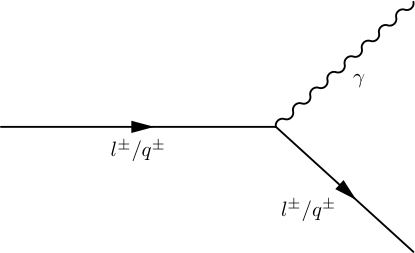
\includegraphics[width=0.49\textwidth]{img/I-1-standard-model/diagram-photon.png}
      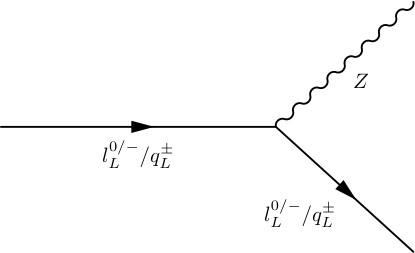
\includegraphics[width=0.49\textwidth]{img/I-1-standard-model/diagram-Z.png} \\
      \vspace*{0.3cm}
      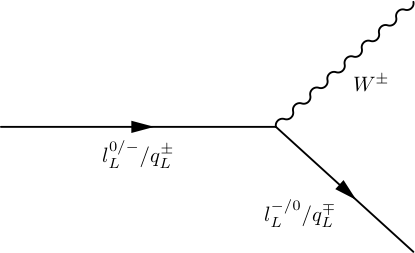
\includegraphics[width=0.49\textwidth]{img/I-1-standard-model/diagram-W.png}
      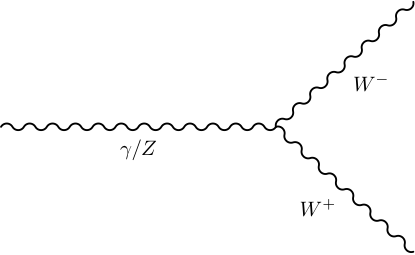
\includegraphics[width=0.49\textwidth]{img/I-1-standard-model/diagram-WZphoton.png}
      \caption{Feynman diagrams representing the interaction of the $ \gamma $, $ Z $ boson, and $ W^\pm $ bosons to fermions. Top-left: coupling of $ \gamma $ to charged particles. Top-right: diagonal coupling of the $ Z $ boson to $ SU(2)_L $ doublets. Bottom-left: non-diagonal coupling of the $ W^\pm $ bosons to $ SU(2)_L $ doublets. Bottom-right: self-coupling of the gauge bosons.}
      \label{fig:I-1-diagram-EWK}
    \end{figure}

  \section{Quantum Chromodynamics}

    QCD uses the $ SU(3)_C $ gauge group to describe the behavior of quarks and gluons, and introduces the notion of color charge. After the observation of particles composed of three identical quarks in the same spin configuration, a new quantum number had to be introduced in order to obey Pauli's exclusion principle. Through their interaction with the $ SU(3)_C $ group, quarks carry a color, arbitrarily labeled red, blue, or green, that is exchanged by the interaction with gluons which carry a color and anti-color combination. However, as given quark configurations were not observed experimentally, a constraint was added and forced hadrons, groups of quarks, to be colorless: either composed of a quark and an antiquark of opposite color for mesons, or composed of three quarks of different colors for baryons. Recently, pentaquarks composed of four quarks and one antiquark have been observed by the Large Hadron Collider Beauty experiment at CERN \cite{Aaij:2015tga}. \\

    Quarks are placed in the fundamental representation of the $ SU(3)_C $ group which are triplets of the same quark flavor with three different colors, while leptons are singlets as they do not interact under QCD. The covariant derivate becomes
    \begin{equation}
      D_\mu = \partial_\mu - \frac{i g_S}{2} G^a_\mu \lambda^a
    \end{equation}
    where $ g_S $ is the strong coupling constant, $ G^a $ are the eight gluon gauge fields, and $ \lambda^a $ are the Gell-Mann matrices. Gluons are massless as they do not interact with the Higgs fields through the EWK symmetry breaking. \\

    The observation of flavor-changing charged current interactions, interactions mediated through a $ W^\pm $ that couple quarks from different $ SU(2)_L $ doublets, lead N. Cabibbo, M. Kobayashi, and T. Maskawa to introduce the concept of mixing matrix for the quarks. They postulated that the eigenstates of quarks that interact with the EWK gauge bosons, the ones that are present in the doublets, are not he eigenstates of mass, thus the physical particles. By introducing a CKM matrix which for each quark redefines a linear combination of the other quarks, they were able to account for the violation of quark flavor in the EWK sector.

  \section{Beyond the Standard Model}

    Although the standard model provides a very accurate description of the QCD and EWK theories it bares some shortcomings in order to be considered to be the theory of everything. \\

    The success of the unification of the weak and electromagnetic forces into a single EWK theory has motivated physicists to unify QCD and EWK into a single force at high energies, described by a new gauge invariance group. This implies a symmetry breaking mechanism similar to the Higgs mechanism at low energies and thus the existence of new particles of high mass undetected as of today. \\

    QCD and EWK theories, although not yet unified, have successfully been combined in the standard model to account for strong, weak, and electromagnetic forces. However, including Einstein's theory of general relativity, which describes gravitational forces, still remains a challenge. Some theories propose to add a new boson to the model, the graviton, to account for gravity but fail to describe all phenomena experimentally observed. To this day, general relativity remains the prominent theory of gravitation, validated by the recent discovery of gravitational waves by the LIGO experiment in February 2016 \cite{PhysRevLett.116.061102}. \\

    Although general relativity provides predictions that have been experimentally tested with great precision, it fails to account for effects such as the excessive rotation speed of galaxies or gravitational lensing. Instead of rewriting Einstein's theory, the existence of dark matter and energy has been postulated which would interact gravitationally but not through any other force. From computation, only 5\% of our universe would be composed of standard model particles while the remaining 95\% would be made of yet unknown matter and energy. Physicists also postulate the existence of a hidden sector, which new exotic particles interact only rarely with ordinary matter and at higher energy scales. \\

    Finally, the standard model as it is written fails to give mass to the neutrinos while experimental results have proven that neutrinos, although very light, carry a mass. Moreover, neutrino oscillations between generations have been observed by Super-Kamiokande in 1998 \cite{Fukuda:1998mi}, meaning that the standard model neutrinos, those placed in the $ SU(2)_L $ doublets are not the mass eigenstates of the particles. \\

    These examples are only a few of the questions that remain open. To answer some of them, physicists need to reach higher energies in order to explore new sectors of physics unaccessible under normal conditions. To reach that goal, powerful machines such as particle colliders have been build over the last century. The latest achievement in this field is the construction of the Large Hadron Collider at CERN which already had a great success with the discovery of the Brout-Englert-Higgs boson.
